\documentclass[10pt,a4paper]{article}
\usepackage[margin=22mm,headheight=27pt]{geometry}
\usepackage[T1]{fontenc}
\usepackage{lmodern,microtype}
\usepackage{graphicx,booktabs,longtable,tabularx,array,amsmath}
\usepackage{tikz}
\usetikzlibrary{arrows.meta,positioning,fit,calc}
\usepackage{listings,needspace,xcolor,fancyhdr,caption}
\usepackage[hidelinks]{hyperref}
\usepackage{xurl}
\definecolor{codegray}{gray}{0.96}
\hypersetup{pdftitle={AEGIS: Data Analysis and Database Design},pdfauthor={Ilias Akritidis, Georgios Mallousis, Vasileios Sevetlidis}}
\pagestyle{fancy}\fancyhf{}
\fancyhead[L]{\small AEGIS: Data Analysis}
\fancyhead[R]{\footnotesize\begin{tabular}{@{}r@{}}ARGUS Open Innovation Challenge 2026\\Track A: Heritage and Citizen Science\end{tabular}}
\fancyfoot[C]{\small\thepage}
\renewcommand{\headrulewidth}{0.3pt}
\setlength{\parskip}{0.35em}\setlength{\parindent}{1em}
\setlength{\emergencystretch}{2em}\setlength{\textfloatsep}{13pt}
\captionsetup{font=small,labelfont=bf}
\newcolumntype{Y}{>{\raggedright\arraybackslash}X}
\lstset{basicstyle=\ttfamily\footnotesize,backgroundcolor=\color{codegray},frame=single,breaklines=true,columns=fullflexible,keepspaces=true,showstringspaces=false}
\tikzset{box/.style={draw=black!65,rounded corners=1pt,align=center,font=\small,inner sep=5pt},flow/.style={-{Latex[length=2mm]},draw=black!75},tag/.style={font=\scriptsize,align=left,fill=white,inner sep=2pt}}
\begin{document}
\raggedbottom
\fontsize{10.5}{13}\selectfont
\begin{center}
{\LARGE\bfseries AEGIS: Data Analysis and Database Design\par}
\vspace{0.5em}{\large Technical Deliverable\par}
\vspace{0.6em}
Ilias Akritidis\textsuperscript{*}, Georgios Mallousis\textsuperscript{*}, Vasileios Sevetlidis\par
\vspace{0.3em}
{\small International Hellenic University, Polytechnic School\\
Department of Computer, Informatics and Telecommunications Engineering\par}
{\small\href{mailto:iliakrit@ihu.gr}{\texttt{iliakrit@ihu.gr}}\quad
\href{mailto:geomallo@ihu.gr}{\texttt{geomallo@ihu.gr}}\quad
\href{mailto:vasiseve@ihu.gr}{\texttt{vasiseve@ihu.gr}}\par}

\end{center}
{\renewcommand{\thefootnote}{\fnsymbol{footnote}}\footnotetext[1]{Ilias Akritidis and Georgios Mallousis contributed equally to this work.}}

% \begin{abstract}
% AEGIS transforms heritage-monitoring records into structured learning activities through a reproducible, rule-based data-analysis pipeline. Risk scenarios, installed instruments, monitoring policies and recorded alarms are integrated with educational mappings to construct missions and explain sensor-network choices. This deliverable specifies the input data model, preparation and selection procedures, derived indicators and resulting application dataset. Recalculation from the retained inputs identifies 99 risk scenarios and reduces 337 alarm records to 90 usable alarms, of which 33 are selected for presentation across five heritage sites. A separate analysis examines the optional PostgreSQL database for gameplay and quiz records, including its constraints, access policies and analytical capabilities. The distinction between source observations, application rules and player-generated records provides the basis for interpreting the results and their limitations.
% \end{abstract}

\section{Purpose and analytical scope}
The analysis supports an educational question: how can a non-specialist connect a heritage site's preservation challenges with the monitoring instruments capable of detecting relevant changes? The resulting dataset represents threats, monitoring networks and interpretable events at Delos, Baltan\'as, Monti Lucretili, Sant'Antonio di Ranverso and Schenkenberg. Missions translate these records into bounded sensor-selection tasks. Recorded alarms provide examples against which proposed networks can be examined.

Two data domains support this process. The heritage domain consists of ARGUS records retrieved through its API and retained as JSON snapshots. The participation domain consists of gameplay and quiz records stored on the device, on a classroom server, or in an optional Supabase PostgreSQL database. The preparation pipeline reads the heritage domain; participation statistics are computed separately in the browser. The SQL schema examined here defines the application's participation store. The ARGUS data model is examined through its API representations.\footnote{Implementation sources: \path{tools/build_game_data.py}, \path{web/src/game/logic.ts}, \path{web/src/community/store.ts}, \path{web/src/community/index.ts}, \path{tools/class_server.py} and \path{supabase/schema.sql}. The analysis concerns the local \texttt{readyToSubmit} branch, with application baseline \texttt{b61c190}. Paths in implementation footnotes are relative to the repository.}

The scope includes record integration, quality screening, alarm selection, mission construction, descriptive participation measures and static database analysis. The analysis uses deterministic application rules. Database findings derive from static examination of the supplied DDL and consuming code. Establishing the configuration, contents and performance of a running Supabase instance requires deployment inspection.

\section{Methodological basis}
CRISP-DM describes an iterative process spanning business understanding, data understanding, preparation, modelling, evaluation and deployment~\cite{crispdm}. These phases organise the AEGIS workflow (Table~\ref{tab:crisp}). Here, modelling consists of explicit transformation and selection rules.

Rahm and Do distinguish schema-level integration issues from instance-level problems such as missing values, invalid values and duplicate records~\cite{rahm2000}. This distinction informs the separation between relational reconstruction, alarm screening and retained quality flags. Filtering establishes suitability for the educational application. Assessing a record's operational validity requires the semantics and requirements of its original monitoring context.

Reproducibility also requires identifying the inputs and procedures associated with a result. Sandve et al. emphasise retaining software, data and intermediate information sufficient to reconstruct computational findings~\cite{sandve2013}. AEGIS retains snapshots, executable transformations, educational mappings and generated analysis notes. Reproduction therefore depends on both the ARGUS records and the version of the application content.

\begin{table}[htbp]
\centering\small
\caption{Organisation of the implemented analysis using CRISP-DM phases.}\label{tab:crisp}
\begin{tabularx}{\linewidth}{@{}>{\raggedright\arraybackslash}p{3.0cm}Y@{}}
\toprule Phase & Application in AEGIS\\\midrule
Understanding the purpose & Relate preservation threats, sensor choices and interpretable alarms for non-specialist users.\\
Understanding the data & Inspect resources, metadata, identifiers, priorities, instrument positions and event types.\\
Preparation & Reconstruct joins, handle duplicate alarms and apply completeness, mapping and plausibility rules.\\
Modelling & Map threats and alarm rules to sensor cards, group alarm episodes and construct missions.\\
Evaluation & Validate references and content; test deterministic output, selection rules, scoring and record handling.\\
Deployment & Publish the gameplay pack; compute participation summaries through the configured record store.\\
\bottomrule
\end{tabularx}
\end{table}

\section{Input data and logical relationships}
\subsection{Retained sources and temporal coverage}
The principal inputs come from \path{snapshot_2026-10-12/}. Ten resources were retrieved between 15:00:44 and 15:02:45 on 12 October 2026, at UTC+03:00. Decision resources are supplied by the retained snapshot of 11 October. Table~\ref{tab:inputs} reports counts recalculated from the files. Each listed file declares \texttt{complete=true}, and its recorded count agrees with the number of retained records.\footnote{Core inputs: \path{snapshot_2026-10-12/*.json}. Supplemental decisions: \path{snapshot/decisions.json} and \path{snapshot/decision-contexts.json}. The fallback is implemented by \texttt{load\_snapshot}; the game derives its displayed core snapshot date from the ten principal resources.}

Completeness describes the retained API retrieval according to its metadata. Historical coverage and the extent of site observations require additional information about the upstream service. The resource timestamps document sequential acquisition. The AD-RT alarm timestamps span 28 August--8 October 2026. The generated notes contain a fixed sentence describing events as an incomplete sample, in conflict with the retained file's completeness flag. Counts reported here use the retained records and their actual metadata.

\begin{table}[htbp]
\centering\small
\caption{Resources used in the retained analysis and their principal roles.}\label{tab:inputs}
\begin{tabularx}{\linewidth}{@{}p{3.6cm}rY@{}}
\toprule Resource & Records & Analytical role\\\midrule
\texttt{assets} & 5 & Heritage-site identity and pilot association.\\
\texttt{asset-states} & 47 & Associate installed devices with heritage assets.\\
\texttt{threats} & 156 & Identify ABC risk scenarios and priorities.\\
\texttt{threat-contexts} & 1,350 & Recover scenario evaluation histories.\\
\texttt{events} & 1,543 & Identify AD-RT alarms and their metadata.\\
\texttt{policies} & 181 & Retrieve policy context and threshold overrides.\\
\texttt{installed-instruments} & 123 & Link registered instruments to installed devices.\\
\texttt{installed-devices} & 117 & Supply asset-state links and position metadata.\\
\texttt{instruments} & 117 & Resolve instrument identity and type.\\
\texttt{instrument-types} & 40 & Map type names to educational sensor cards.\\
\texttt{decisions} & 219 & Supply recorded recommendations.\\
\texttt{decision-contexts} & 217 & Associate recommendations with alarm context.\\
\bottomrule
\end{tabularx}
\end{table}

The analysis operates on scenarios and derived monitoring events. The short retained readings series and the undocumented \texttt{sensor\_coverage} field lie outside the selected inputs. Alarm reconstruction from original sensor time series would require a dedicated analysis.

\subsection{Reconstruction of the heritage data model}
API metadata may be a JSON-encoded string, an object or null. Parsing exposes the scenario, pilot, alarm and evaluation attributes. Unparseable metadata is retained internally as an unparsed value. Preparation and validation check the required relationships and application references after parsing.

An installed-instrument record links to an installed device and an instrument. The device links to an asset state, which identifies the heritage asset. The instrument links to its type. This chain assigns each instrument to a site and then to a sensor card. Pilot identifiers in scenario metadata are matched to asset codes, with exactly one matching asset required. Risk histories are grouped by \texttt{scenario\_key}. Recommendations are associated with alarms through pilot, original rule and timestamp. These logical relationships are reconstructed from the API representations. Verification of physical foreign-key constraints would require access to the ARGUS database definition.

\subsection{Educational mappings and provenance}
Sensor-card definitions specify labels, costs and instrument-type associations. Threat mappings identify primary and supporting cards, first by scenario and otherwise by risk category. Rule mappings specify sensor combinations, feature-name patterns and any rule-specific plausibility bounds. Monument content supplies explanations, curated missions and preferred replay events.\footnote{Content definitions: \path{content/sensor_cards.json}, \path{content/threat_sensor_map.json}, \path{content/rule_sensor_map.json}, \path{content/coins.json} and \path{content/monuments/*.json}.}

The generated dataset distinguishes ARGUS-derived fields from authored content through provenance descriptions and \texttt{authored} or \texttt{needs\_review} flags. Prices, sensor mappings, narrative explanations and illustrative deterioration rates originate in the application's educational configuration. Figure~\ref{fig:pipeline} presents the separation of inputs, transformations and outputs.
\begin{figure}[htbp]
\centering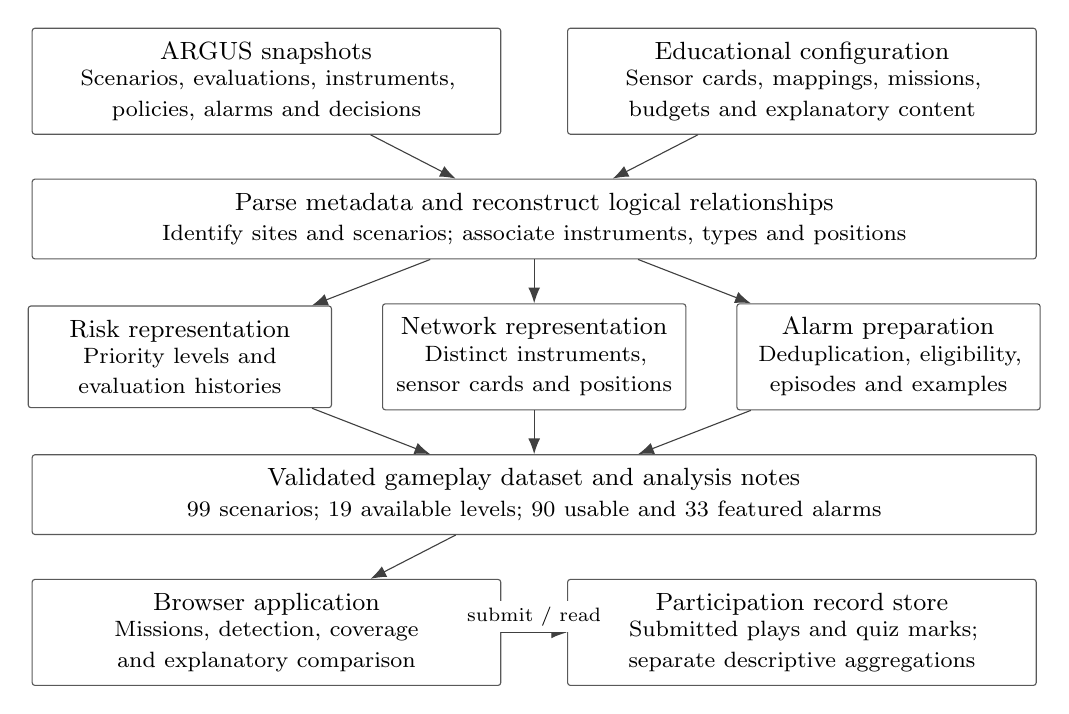
\begin{tikzpicture}
\node[box,text width=5.6cm] (argus) at (-3.4,0) {ARGUS snapshots\\\footnotesize Scenarios, evaluations, instruments,\\policies, alarms and decisions};
\node[box,text width=5.6cm] (content) at (3.4,0) {Educational configuration\\\footnotesize Sensor cards, mappings, missions,\\budgets and explanatory content};
\node[box,text width=12.4cm] (prepare) at (0,-1.75) {Parse metadata and reconstruct logical relationships\\\footnotesize Identify sites and scenarios; associate instruments, types and positions};
\node[box,text width=3.5cm] (risk) at (-4.5,-3.5) {Risk representation\\\footnotesize Priority levels and\\evaluation histories};
\node[box,text width=3.5cm] (network) at (0,-3.5) {Network representation\\\footnotesize Distinct instruments,\\sensor cards and positions};
\node[box,text width=3.5cm] (alarm) at (4.5,-3.5) {Alarm preparation\\\footnotesize Deduplication, eligibility,\\episodes and examples};
\node[box,text width=12.4cm] (output) at (0,-5.25) {Validated gameplay dataset and analysis notes\\\footnotesize 99 scenarios; 19 available levels; 90 usable and 33 featured alarms};
\node[box,text width=5.6cm] (browser) at (-3.4,-7) {Browser application\\\footnotesize Missions, detection, coverage\\and explanatory comparison};
\node[box,text width=5.6cm] (player) at (3.4,-7) {Participation record store\\\footnotesize Submitted plays and quiz marks;\\separate descriptive aggregations};
\draw[flow] (argus)--(prepare);
\draw[flow] (content)--(prepare);
\foreach \n in {risk,network,alarm} {
  \draw[flow] (prepare)--(\n);
  \draw[flow] (\n)--(output);
}
\draw[flow] (output)--(browser);
\draw[flow] (browser)--node[tag,above]{submit / read}(player);
\end{tikzpicture}

\caption{Data preparation and consumption. Participation records support browser-side descriptive analysis through the configured community store.}\label{fig:pipeline}
\end{figure}

\section{Data preparation and selection}
\subsection{Risk scenarios and evaluation histories}
Records of kind \texttt{abc\_risk\_scenario} supply the risk scenarios. The inputs contain 99 scenarios. Priority labels map directly to the five levels: 30 low, 20 medium, 16 high, 23 extreme and 10 catastrophic. The dataset preserves the source ABC components and magnitude.

The builder recognises 1,133 records of kind \texttt{ira\_threat\_evaluation}, associated with 51 scenario keys. Evaluations are ordered by source timestamps. Consecutive evaluations above \texttt{inactive} are summarised as state intervals, with the largest probability within each interval retained. One scenario has a raised history in these inputs: wind erosion at the House of the Masks on Delos, at the \texttt{watch} state. These results describe the recorded evaluation states within the retained period. Site-wide preservation risk requires assessment across the relevant evidence and time horizon.

\subsection{Instrument identity and position}
The 123 installation records resolve to 117 distinct instruments. Grouping by instrument identifier avoids counting repeated registrations as separate instruments. At Ranverso, 26 records describe 20 distinct instruments. Instruments are subsequently grouped by educational card for comparison with a proposed network. Coordinate pairs group the positioned instruments into 74 site-specific map points. Temporary positions, positions inherited from a sibling sensor and virtual instruments carry corresponding flags. Map points group instruments sharing coordinates.

\subsection{Alarm identity and duplicate handling}
The event file contains 337 AD-RT alarm records, alongside 1,134 IRA evaluation events and 72 EOP completion events. Alarm records comprise 217 expert-rule events (\texttt{EK}) and 120 model-derived events (\texttt{DL}).

Within each site, alarm identity is reconstructed using type, original rule, timestamp and the ordered variable-name sequence. Where no variable list is supplied, sorted feature-contribution names are used. Records are processed by increasing event identifier; the first supplies the retained values and subsequent matches contribute their identifiers. Differences in variable values set a quality flag. The resulting 257 unique alarms reflect grouping by this explicit identity key, including groups containing value variants.\footnote{Alarm preparation: \texttt{build\_alarms}, \texttt{dl\_rule}, \texttt{policy\_thresholds} and \texttt{link\_instruments} in \path{tools/build_game_data.py}.}

\subsection{Interpretability and completeness}
Expert-rule alarms retain their rule and variable. For a DL alarm, the largest supplied feature contribution identifies the principal signal. The alarm proceeds only if this contribution is at least 0.30 and its feature name matches a configured sensor-rule mapping. The 0.30 contribution threshold is an application screening parameter whose explanatory suitability requires evaluation against the upstream model.

For DL alarms, the analysed value is the model's anomaly score and the comparison limit is its anomaly threshold. The feature name supplies the sensor association, and the value retains its anomaly-score semantics. Subsequent processing requires a mapped rule, exactly one represented variable, numeric value and threshold, and a non-zero threshold. The inputs lose 66 unique alarms at the DL interpretation stage and 24 at the rule/completeness stage.

\subsection{Plausibility and retained quality information}
Physical range screening applies to EK measurements: humidity and soil moisture from 0 to 100, rain from 0 to 1,000, and temperature from $-50$ to $60$. Rule-specific bounds further constrain derived quantities, including daily temperature range and one-hour temperature change. Exact zero humidity or soil moisture is treated as a suspect dropout. These eligibility rules depend on assumed variable semantics and units. Sensor-fault diagnosis requires calibration against the relevant instruments and operating conditions. DL anomaly scores undergo the applicable rule-specific checks.

This stage excludes 77 further alarms: 31 for humidity range, 19 for temperature range, 18 for the daily temperature-range rule, six for the one-hour change rule, and three for zero soil moisture. The resulting set contains 90 usable alarms. Disagreement with a current policy threshold and conflicting duplicate values are retained as flags alongside the selected values. The 37 AD-RT expert-rule policies provide current threshold context. Establishing the policy in force at a historical event requires the corresponding policy history.

\subsection{Episode construction and featured examples}
Usable alarms are grouped by mapped rule and ordered by timestamp. A gap strictly greater than 48 hours starts a new episode. The displayed threshold multiple is
\begin{equation}
r(v,\tau)=
\begin{cases}
v/\tau,&v\geq\tau,\\
\tau/v,&v<\tau,\ v\neq0.
\end{cases}
\end{equation}
The ratio is undefined for a zero value in the second case. Its analytical role is to order examples within the selection procedure. Interpretation in terms of physical damage, cross-sensor risk or prediction confidence would require a separately calibrated relationship.

An episode with at least three observations is flagged as approximately flat when
\begin{equation}
\bar v\neq0
\quad\text{and}\quad
\frac{\max(v)-\min(v)}{|\bar v|}<0.02.
\end{equation}
The first, peak and last alarm of each episode are selected, with roles combined when they identify the same alarm. Additional high-ratio examples bring the selection towards five alarms where sufficient records exist. A ten-alarm cap per site prioritises peaks before other roles. Flat-signal flags remain in the data. Level-replay selection filters out examples carrying a flat-signal flag. These operations produce a purposive selection of 33 illustrative alarms.

\begin{figure}[htbp]
\centering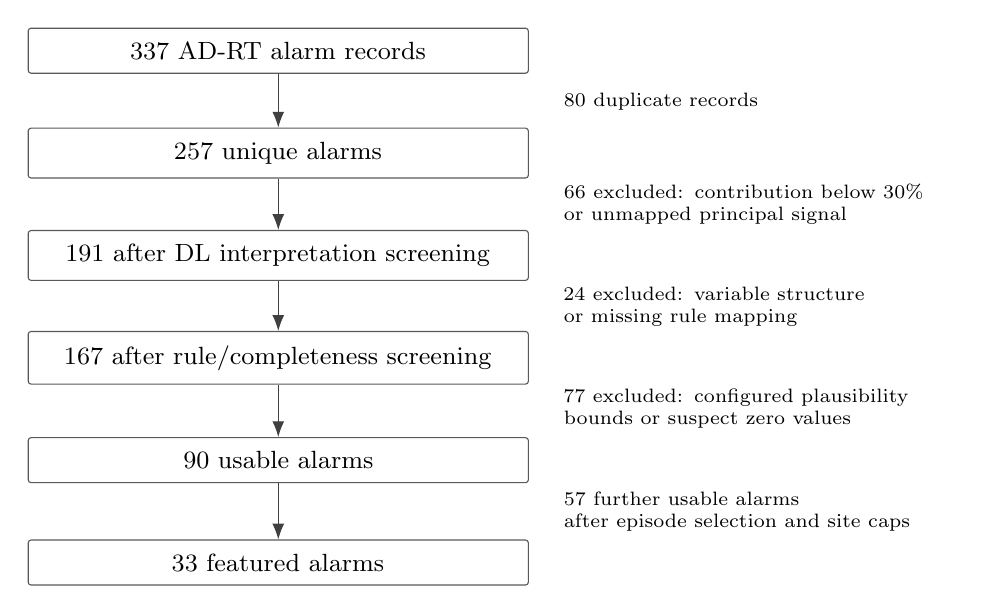
\begin{tikzpicture}
\node[box,text width=6cm] (raw) at (0,0) {337 AD-RT alarm records};
\node[box,text width=6cm] (unique) at (0,-1.3) {257 unique alarms};
\node[box,text width=6cm] (mapped) at (0,-2.6) {191 after DL interpretation screening};
\node[box,text width=6cm] (complete) at (0,-3.9) {167 after rule/completeness screening};
\node[box,text width=6cm] (usable) at (0,-5.2) {90 usable alarms};
\node[box,text width=6cm] (featured) at (0,-6.5) {33 featured alarms};
\draw[flow] (raw)--(unique);
\draw[flow] (unique)--(mapped);
\draw[flow] (mapped)--(complete);
\draw[flow] (complete)--(usable);
\draw[flow] (usable)--(featured);
\node[tag,text width=5.2cm,anchor=west] at (3.55,-0.65) {80 duplicate records};
\node[tag,text width=5.2cm,anchor=west] at (3.55,-1.95) {66 excluded: contribution below 30\%\\or unmapped principal signal};
\node[tag,text width=5.2cm,anchor=west] at (3.55,-3.25) {24 excluded: variable structure\\or missing rule mapping};
\node[tag,text width=5.2cm,anchor=west] at (3.55,-4.55) {77 excluded: configured plausibility\\bounds or suspect zero values};
\node[tag,text width=5.2cm,anchor=west] at (3.55,-5.85) {57 further usable alarms\\after episode selection and site caps};
\end{tikzpicture}

\caption{Sequential alarm eligibility and presentation selection. Exclusions apply to the preceding retained set. A further 57 usable alarms remain outside the featured selection.}\label{fig:funnel}
\end{figure}

\section{Results and construction of learning activities}
\subsection{Distribution across heritage sites}
Table~\ref{tab:results} reports the recalculated site-level results. Overall, 90 of 257 unique alarms pass the eligibility rules (35.0\%), and 33 of those 90 are featured (36.7\%). These proportions describe selection on the retained dataset. Estimating detector accuracy, event prevalence or instrument reliability requires reference outcomes and an appropriate sampling design.
\begin{table}[htbp]
\centering\small
\caption{Observed pipeline results. Exclusions are counted after deduplication.}\label{tab:results}
\begin{tabular}{@{}lrrrrrr@{}}
\toprule Site & Scenarios & Raw & Unique & Excluded & Usable & Featured\\\midrule
Delos & 36 & 46 & 37 & 6 & 31 & 8\\
Baltan\'as & 7 & 41 & 32 & 32 & 0 & 0\\
Monti Lucretili & 19 & 135 & 97 & 81 & 16 & 10\\
Ranverso & 26 & 101 & 81 & 47 & 34 & 7\\
Schenkenberg & 11 & 14 & 10 & 1 & 9 & 8\\\midrule
Total & 99 & 337 & 257 & 167 & 90 & 33\\
\bottomrule
\end{tabular}
\end{table}

At Baltan\'as, 26 unique DL alarms fail the principal-contribution criterion and six have an unmapped principal signal. These screening outcomes account for the site's empty replay selection. The retained records document the occurrence of alarms. The site remains playable through preservation scenarios and network-design activities.

\subsection{Mission generation and scoring}
The content provides 19 available levels: five at Delos, three each at Baltan\'as and Monti Lucretili, and four each at Ranverso and Schenkenberg. A mission contains three scenarios, using curated selections when present. Automatic selection otherwise traverses the requested priority followed by lower and higher priorities, using the builder's magnitude ordering within each group and avoiding repeated descriptions and scenarios without mapped cards. A curated replay specification is used where available; otherwise an eligible peak is preferred.

Detection is represented as a conjunction of sensor groups: the network must include at least one card from every required group. Coverage is full when a primary card is present, partial when only a supporting card is present, and absent otherwise. The score assigns 20 points to full coverage and eight to partial coverage, 25 to detection where a replayable alarm exists, and up to 15 to expenditure on useful cards. The total is normalised to the applicable components:
\begin{equation}
S=\operatorname{round}\!\left(100\,\frac{20F+8P+A+E}{20N+25I+15}\right),
\end{equation}
where $N$ is the number of scorable threats, $F$ and $P$ are full and partial coverage counts, $I$ indicates whether an alarm component applies, $A$ is either 0 or 25 when applicable and zero otherwise, and $E$ is the rounded efficiency component. At sites with an empty replay selection, the score is calculated from threat coverage and efficiency.\footnote{Scoring, sensor-group detection, network comparison and multi-day selection: \path{web/src/game/logic.ts}. Score labels use thresholds 85, 60 and 30, which define the application's educational feedback categories. Establishing their relationship to learning outcomes requires empirical evaluation.}

Comparison with ARGUS's installed network provides descriptive feedback through the network-comparison view. Multi-day gameplay reuses recorded alarms for up to seven days, beginning with the level's event. Illustrative deterioration effects support educational interpretation. Conservation forecasting requires a validated predictive model. The separate recent-data feed reuses the published alarm filter; acquisition and freshness are specified in the API workflow deliverable.\footnote{Companion deliverable: \path{docs/submission/api-workflow/main.tex}. Filter contract: \texttt{alarm\_filter} in \path{web/public/data/game_data.json}.}

\subsection{Published data contract}
The generated \path{web/public/data/game_data.json} uses schema version 3. It contains snapshot metadata, provenance, card and rule definitions, alarm-screening parameters, quiz and observation content, and per-site scenarios, levels, instrument summaries, positions and featured alarms. Explanatory material and spatial references accompany these fields. The retained file occupies 384,489 bytes; the builder's default JSON serialisation is approximately 304.8~KiB. This size excludes the remaining application, imagery, audio and three-dimensional assets.

The accompanying \path{docs/data_notes.md} records counts, exclusions, examples and assumptions. Both outputs agree with fresh execution against the retained inputs. Automatic selection of the newest snapshot means that reproducing these results requires explicitly selecting the dated input directory, together with the original supplemental snapshot and the same content files.

\section{Participation database}
\subsection{Schema and analytical units}
The shared store is defined by \path{supabase/schema.sql}. It creates \texttt{public.plays} and \texttt{public.quizzes}, each with a generated \texttt{bigint} identity primary key. A play row records one submitted gameplay result; a quiz row records one submitted post-game quiz with an optional pre-game response array. The two tables are defined independently. Foreign-key relationships to users, missions and ARGUS resources remain undefined in the supplied schema.

The shared \texttt{monument}, \texttt{class\_code} and \texttt{day} attributes provide grouping dimensions. Session-level association between a play and a quiz requires an additional shared identifier. Joining on the grouping dimensions can produce multiple row combinations. Pre/post responses are paired within each quiz row, supporting comparison at the quiz-submission level. Figure~\ref{fig:database} shows the implemented schema boundary.

PostgreSQL supports relational constraints together with \texttt{jsonb} documents~\cite{pgjson}. AEGIS keeps stable analytical dimensions in scalar columns and represents sensor selections and quiz marks as variable-length structures. The supplied constraints define only part of the intended record semantics (Tables~\ref{tab:plays} and~\ref{tab:quizzes}).
\begin{figure}[htbp]
\centering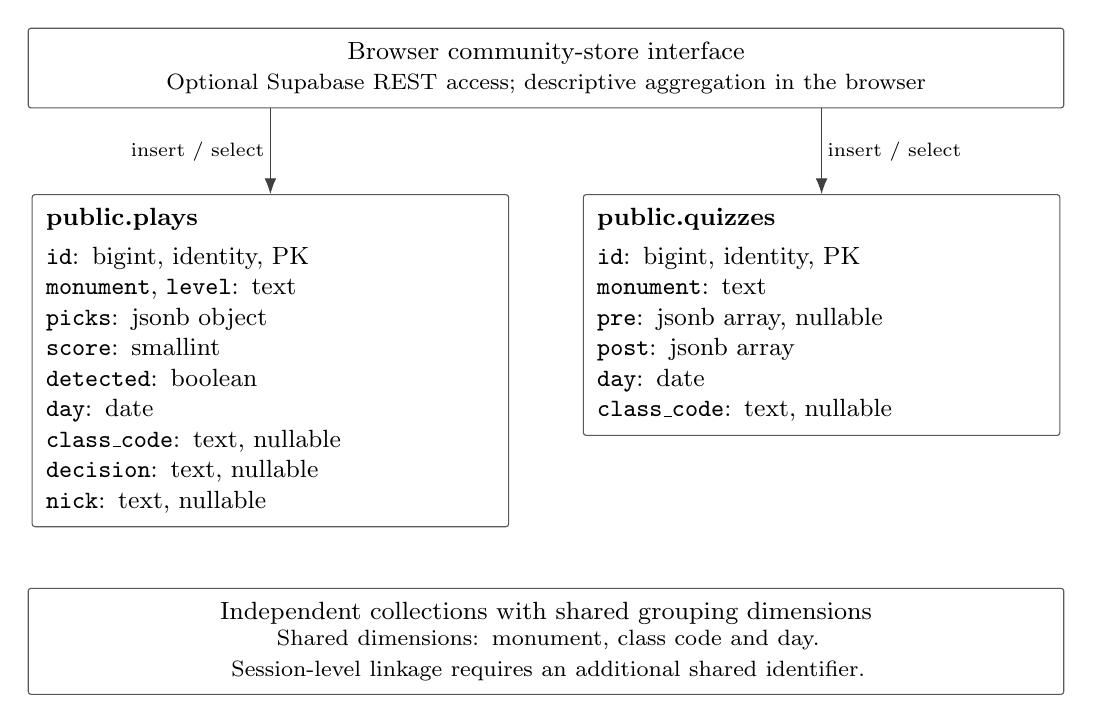
\begin{tikzpicture}
\node[box,text width=12.8cm] (client) at (0,0) {Browser community-store interface\\\footnotesize Optional Supabase REST access; descriptive aggregation in the browser};
\node[box,text width=5.7cm,align=left,anchor=north] (plays) at (-3.5,-1.6) {\textbf{public.plays}\\[3pt]
\texttt{id}: bigint, identity, PK\\
\texttt{monument}, \texttt{level}: text\\
\texttt{picks}: jsonb object\\
\texttt{score}: smallint\\
\texttt{detected}: boolean\\
\texttt{day}: date\\
\texttt{class\_code}: text, nullable\\
\texttt{decision}: text, nullable\\
\texttt{nick}: text, nullable};
\node[box,text width=5.7cm,align=left,anchor=north] (quizzes) at (3.5,-1.6) {\textbf{public.quizzes}\\[3pt]
\texttt{id}: bigint, identity, PK\\
\texttt{monument}: text\\
\texttt{pre}: jsonb array, nullable\\
\texttt{post}: jsonb array\\
\texttt{day}: date\\
\texttt{class\_code}: text, nullable};
\draw[flow] (client.south -| plays.north)--node[tag,left]{insert / select}(plays.north);
\draw[flow] (client.south -| quizzes.north)--node[tag,right]{insert / select}(quizzes.north);
\node[box,text width=12.8cm,anchor=north] at (0,-6.6) {Independent collections with shared grouping dimensions\\\footnotesize Shared dimensions: monument, class code and day.\\Session-level linkage requires an additional shared identifier.};
\end{tikzpicture}

\caption{Participation database and consumers. Each table has an independent primary key. Monument, class code and day support grouping within each collection.}\label{fig:database}
\end{figure}

\begin{table}[htbp]
\centering\small
\caption{Fields and constraints of \texttt{public.plays}.}\label{tab:plays}
\begin{tabularx}{\linewidth}{@{}p{2.1cm}p{2.1cm}Y@{}}
\toprule Field & SQL type & Meaning and declared constraint\\\midrule
\texttt{id} & \texttt{bigint} & Generated identity; primary key.\\
\texttt{monument} & \texttt{text} & Required; 3--20 lowercase ASCII letters. Validation checks the identifier's syntax.\\
\texttt{level} & \texttt{text} & Required; one of low, medium, high, extreme or catastrophic.\\
\texttt{picks} & \texttt{jsonb} & Required object; stored size below 2,000 bytes. Entry-level semantics depend on client validation.\\
\texttt{score} & \texttt{smallint} & Required; client-calculated integer from 0 to 100.\\
\texttt{detected} & \texttt{boolean} & Required; client-reported detection outcome.\\
\texttt{day} & \texttt{date} & Required; 1 January 2026 through the database's current date plus one day when checked.\\
\texttt{class\_code} & \texttt{text} & Optional; six uppercase characters from the configured unambiguous alphabet.\\
\texttt{decision} & \texttt{text} & Optional; 2--30 lowercase letters or underscores. Validation checks the identifier's syntax.\\
\bottomrule
\end{tabularx}
\end{table}

\begin{table}[htbp]
\centering\small
\caption{Fields and constraints of \texttt{public.quizzes}.}\label{tab:quizzes}
\begin{tabularx}{\linewidth}{@{}p{2.1cm}p{2.1cm}Y@{}}
\toprule Field & SQL type & Meaning and declared constraint\\\midrule
\texttt{id} & \texttt{bigint} & Generated identity; primary key.\\
\texttt{monument} & \texttt{text} & Required; same syntactic site rule as \texttt{plays}.\\
\texttt{pre} & \texttt{jsonb} & Optional array of at most 20 elements.\\
\texttt{post} & \texttt{jsonb} & Required array of at most 20 elements.\\
\texttt{day} & \texttt{date} & Required; same date window as \texttt{plays}.\\
\texttt{class\_code} & \texttt{text} & Optional; same six-character pattern as \texttt{plays}.\\
\bottomrule
\end{tabularx}
\end{table}

\subsection{Integrity, indexes and schema evolution}
PostgreSQL provides primary keys, foreign keys, uniqueness, non-null requirements and check constraints as distinct integrity mechanisms~\cite{pgconstraints}. The DDL combines these mechanisms selectively. Identity keys distinguish stored rows. Repeated submissions of the same logical result receive independent row identities. The declared checks permit arbitrary keys and values within the bounded \texttt{picks} object. Quiz arrays may be empty, contain non-boolean elements or have unequal lengths. Enforcing the intended card and response semantics for direct submissions requires additional database constraints.

Three explicit indexes support common filters: \texttt{plays(monument, level)}, \texttt{plays(class\_code)} and \texttt{quizzes(class\_code)}. Primary keys additionally provide identifier indexes. JSON-content indexing and materialised aggregation remain available as possible schema extensions. The REST reader requests selected fields ordered by descending identifier, with a limit of 2,000 rows. Summaries concern the returned subset, whose size also depends on service configuration. Database-wide analysis requires complete retrieval or server-side aggregation. Query-plan inspection and performance measurement lie outside this assessment.

Compatibility statements add \texttt{decision} and \texttt{nick} columns to older projects and replace the nickname check. The browser retries an affected play operation without \texttt{nick} following HTTP 400, accommodating a deployment lacking that column. The HTTP status code triggers this compatibility behaviour. Confirmation of the deployed schema requires direct inspection.\footnote{DDL and indexes: \path{supabase/schema.sql}. REST column selection, descending order, requested limit and nickname compatibility: \texttt{SupabaseCommunityStore} in \path{web/src/community/store.ts}.}

\subsection{Access model and identity semantics}
Row-level security is enabled on both tables. The supplied policies allow the \texttt{anon} role to select all rows and insert rows satisfying table constraints. The script defines policies for selection and insertion; update and delete operations remain subject to PostgreSQL's default-deny behaviour for the anonymous role under this policy set. PostgreSQL evaluates row policies in addition to ordinary privileges; roles with bypass rights and normally table owners are outside that restriction~\cite{pgrls}. Explicit grants, additional existing policies and project-level settings require deployment inspection. This analysis describes the access configuration expressed in the supplied DDL.

The class code is an equality filter in application requests. The select policy permits access to rows across classes. Establishing student or teacher identity requires an authenticated submission mechanism. Scores retain the status of client-reported gameplay results.

The nickname format permits a user-chosen name and a six-character suffix derived in the browser from that name and a password. The submitted nickname contains the chosen name and derived suffix; the password remains in the browser-side computation. Legacy records may use an animal-number label. These formats support leaderboard grouping. Authentication and anonymity require assessment of the complete identity and data-handling design. A chosen name can itself contain identifying information. The schema's introductory comment labels the records anonymous. Privacy assessment should account for the permitted user-chosen names.\footnote{Nickname construction and normalisation: \path{web/src/community/nickname.ts}; optional account flow: \path{web/src/community/account.ts}. Password-storage security and provider logging require separate deployment assessment.}

\subsection{Device, classroom and shared storage}
The default device store retains up to 500 records of each local collection and uses in-memory fallback when browser storage is unavailable. The classroom server writes JSON Lines files, retains up to 50,000 records per file and returns at most the newest 5,000 matching records. It defaults to loopback access, with LAN operation enabled explicitly.

Classroom validation applies the following entry-level checks: sensor selections are limited to 40 entries with integer counts from 1 to 99, and quiz marks must be non-empty boolean arrays of at most 20 elements. Catalogue membership requires additional validation beyond the field-name patterns. Each storage mode applies its documented acceptance rules to the shared record contract.

When shared storage is configured, a local copy and pending queue support retry and fallback. Reads can switch to local records after a shared-store failure. Each successful insertion creates a new row, and an uncertain network outcome followed by retry can produce repeated records. Idempotent submission handling would require a stable submission key and an associated uniqueness constraint. Statistics describe the active storage scope and count submitted records.

\section{Participation measures and interpretation}
For $n$ returned play records, the browser computes mean score, the fraction reporting successful detection, and the proportion of networks containing each sensor card:
\begin{equation}
\bar S=\frac{1}{n}\sum_{i=1}^{n}S_i,\qquad
p_{\mathrm{det}}=\frac{1}{n}\sum_{i=1}^{n}\mathbf{1}(d_i),\qquad
p_c=\frac{1}{n}\sum_{i=1}^{n}\mathbf{1}(q_{ic}>0).
\end{equation}
Here $q_{ic}$ is the selected quantity of card $c$. The last measure expresses the frequency with which networks include a card. Decision counts include only records with a decision. Empty collections return zero for means and shares. The accompanying record count identifies empty collections.

For quiz summaries, the paired set contains rows with a pre-game array. Mean pre- and post-game correct-answer counts use that same set. Per-question comparison additionally requires both arrays to match the requested question count. The general summary accepts the recorded array lengths. The per-question analysis uses its specified question count to establish a common response structure.\footnote{Aggregations: \texttt{summarize}, \texttt{decisionCounts}, \texttt{summarizeQuiz} and \texttt{quizByQuestion} in \path{web/src/community/store.ts}.}

The stored quiz marks support descriptive comparison within each submission. Analysis of quiz version, individual answer choices, session identity, intervention exposure and verified participants would require additional fields. Repeat play, selective completion, differing missions, changes in quiz content and bounded retrieval can affect comparisons. Estimating causal learning effects and their persistence requires an appropriate evaluation design and follow-up observations. The user-experience questionnaire cited in the abstract forms a separate dataset. The available participation evidence comprises the schema and consuming code; analysis of player sample sizes and outcomes requires populated records.

\section{Reproduction and verification}
\subsection{Reconstructing the retained analysis}
The core builder requires Python 3.9 or later and uses the standard library. These commands select the retained snapshot explicitly; the first validates without writing and the second regenerates output:
\begin{lstlisting}
python3 -I tools/build_game_data.py --snapshot snapshot_2026-10-12 --check
python3 -I tools/build_game_data.py --snapshot snapshot_2026-10-12
\end{lstlisting}
The original snapshot remains necessary for supplemental decisions, and the corresponding content, translation and spatial files must be retained. Acquisition of a new snapshot is unnecessary for reproducing these results. Newer snapshots or changed mappings can legitimately produce different output.

Read-only SQL inspection queries appear in Appendix~\ref{app:sql}. They provide a procedure for comparing a deployed database with the supplied schema. Execution against a remote service remains a deployment verification step. Applying DDL or changing access policies lies outside this verification.

% \subsection{Executed checks}
% Checks on 25 October 2026 passed 41 Python data-builder tests and 16 classroom-server tests, together with 13 browser community-store tests, 14 multi-day gameplay tests and 41 scoring/logic tests: 125 targeted tests in total. The data-pack validator also passed, with five playable sites and 485 of 485 text keys present in each Italian, Spanish and German translation pack. Linguistic quality requires language review.\footnote{Python checks: \path{tools/tests/test_build_game_data.py} and \path{tools/tests/test_class_server.py}. Browser checks: \path{web/tests/community.test.ts}, \path{web/tests/week.test.ts} and \path{web/tests/logic.test.ts}.}

% These checks cover deterministic repeated builds, agreement with retained JSON, unchanged snapshot files, alarm and mission consistency, record validation, classroom persistence and aggregation behaviour. Fresh computation also reproduced the analysis notes. The SQL assessment consists of static examination of the schema and its clients. Execution in PostgreSQL and verification of deployed policies, grants, cloud availability, record completeness and submission authenticity remain deployment-level assessment tasks.

\section{Limitations and conclusion}
The heritage analysis depends on source semantics and units and on application mappings requiring expert review. Duplicate resolution retains the first matching record and flags value conflicts. Episode boundaries, screening ranges, feature-contribution eligibility and selection caps are explicit configuration choices, whose effects require sensitivity analysis. Selection favours interpretable examples. Estimation of environmental-event frequency and upstream detector performance requires a suitable sampling design and reference outcomes. The participation database provides a compact record of submitted choices and quiz marks. Its schema supports descriptive summaries of submitted records. Session linkage, authenticated participant counting, harmonised validation and duplicate prevention require additional schema and application mechanisms. These conditions define the scope of interpretation. Within this scope, AEGIS provides a traceable transformation from retained monitoring records to 19 playable levels, with source-linked scenarios, instrument comparisons and selected alarm examples. Separating heritage observations, educational configuration and participation records makes the analytical basis inspectable and supports subsequent expert review and evaluation.

\clearpage
\begin{thebibliography}{9}
\small
\bibitem{crispdm} IBM, \emph{IBM SPSS Modeler CRISP-DM Guide}, version 18.5.0, ch.~1. \url{https://www.ibm.com/docs/en/SS3RA7_18.5.0/pdf/ModelerCRISPDM.pdf}.
\bibitem{rahm2000} E. Rahm and H.~H. Do, \emph{Data Cleaning: Problems and Current Approaches}, IEEE Data Engineering Bulletin, vol.~23, no.~4, pp.~3--13, 2000. \url{https://pubs.dbs.uni-leipzig.de/dc/files/Rahm2000DataCleaningProblemsand.pdf}.
\bibitem{sandve2013} G.~K. Sandve, A. Nekrutenko, J. Taylor and E. Hovig, \emph{Ten Simple Rules for Reproducible Computational Research}, PLOS Computational Biology, vol.~9, no.~10, e1003285, 2013. \url{https://doi.org/10.1371/journal.pcbi.1003285}.
\bibitem{pgjson} PostgreSQL Global Development Group, \emph{PostgreSQL 17 Documentation}, sec.~8.14, JSON Types. \url{https://www.postgresql.org/docs/17/datatype-json.html}.
\bibitem{pgconstraints} PostgreSQL Global Development Group, \emph{PostgreSQL 17 Documentation}, sec.~5.5, Constraints. \url{https://www.postgresql.org/docs/17/ddl-constraints.html}.
\bibitem{pgrls} PostgreSQL Global Development Group, \emph{PostgreSQL 17 Documentation}, sec.~5.9, Row Security Policies. \url{https://www.postgresql.org/docs/17/ddl-rowsecurity.html}.
\end{thebibliography}
\clearpage\appendix
\section{Read-only database inspection}\label{app:sql}
These PostgreSQL queries provide inspection procedures for an authorised database connection. Inspection of policies should be accompanied by inspection of table grants and the effective API role.
\begin{lstlisting}[language=SQL]
-- Column types and nullability.
SELECT table_name, column_name, data_type, is_nullable
FROM information_schema.columns
WHERE table_schema = 'public'
  AND table_name IN ('plays', 'quizzes')
ORDER BY table_name, ordinal_position;

-- All policies, including any added outside the supplied DDL.
SELECT tablename, policyname, roles, cmd, qual, with_check
FROM pg_policies
WHERE schemaname = 'public'
  AND tablename IN ('plays', 'quizzes');

-- Index definitions.
SELECT tablename, indexname, indexdef
FROM pg_indexes
WHERE schemaname = 'public'
  AND tablename IN ('plays', 'quizzes');
\end{lstlisting}
A database-side summary operates on all rows visible to the executing role and describes submissions and client-reported outcomes:
\begin{lstlisting}[language=SQL]
SELECT monument, level,
       COUNT(*) AS submissions,
       AVG(score) AS mean_submitted_score,
       COUNT(*) FILTER (WHERE detected)::numeric
         / NULLIF(COUNT(*), 0) AS reported_detection_share
FROM public.plays
GROUP BY monument, level
ORDER BY monument, level;
\end{lstlisting}
The queries analyse each table independently. A session-level join would require a shared session identifier.
\end{document}
